% Rachel: parity experiment figures, column width, placed in-line ([H]) at the end of the section.
% \input from a1.tex after \end{multicols}. Regenerate: python -m experiments.parity_* (--plot-only).
% Numbers behind each figure: figures/parity_*.md.

\begin{figure}[H]
\centering
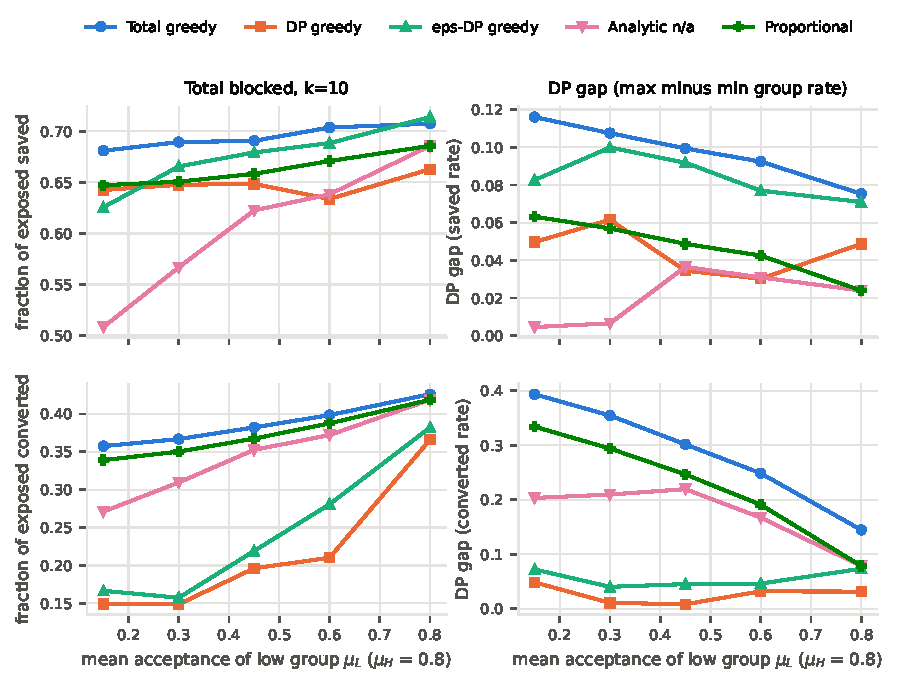
\includegraphics[width=\columnwidth]{figures/parity_sweep_acceptance.pdf}
\caption{Parity experiment A: total blocked (left) and DP gap (right) at $k=10$ as the low group's mean acceptance $\mu_L$ falls. Top: \emph{saved}; bottom: \emph{converted}. Setup in Section~\ref{sec:setup}. DP greedy maximizes $F_\lambda$ with $\lambda=2$; $\varepsilon$-DP greedy uses $\varepsilon=0.05$; Analytic sets $k_g\propto n_g/\bar a_g$ and Proportional $k_g\propto n_g$, each taking the highest-degree nodes in each group.}
\label{fig:parity-accept}
\end{figure}

\begin{figure}[H]
\centering
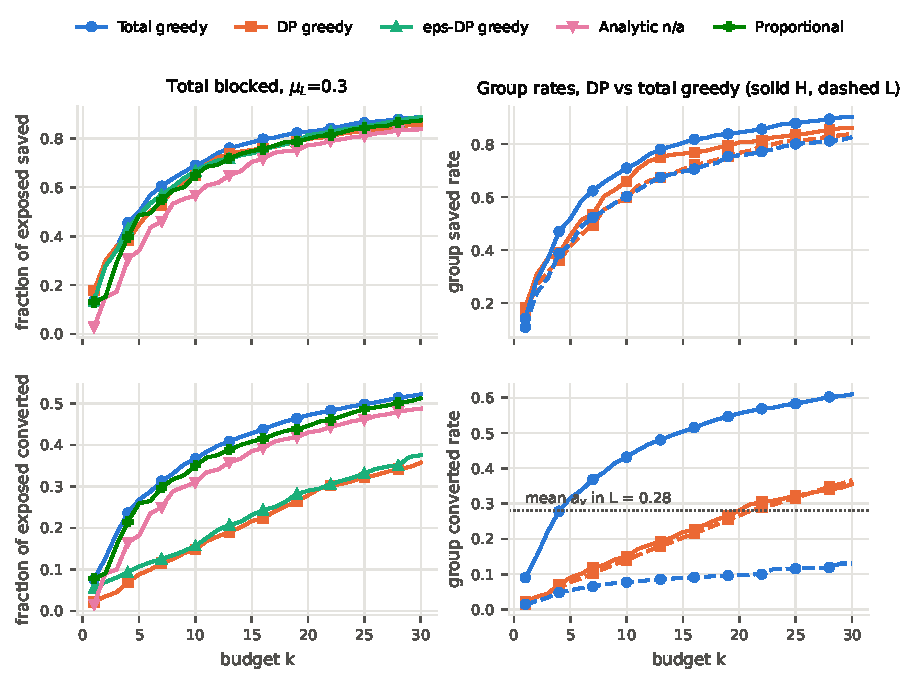
\includegraphics[width=\columnwidth]{figures/parity_sweep_budget.pdf}
\caption{Parity experiment B: budget $k=1,\dots,30$ at $\mu_L=0.3$ (realized mean acceptance 0.81 in $H$, 0.28 in $L$). Left: total blocked by each method. Right: per-group rates for DP greedy and total greedy (solid $H$, dashed $L$). The dotted line is $L$'s mean acceptance, which bounds $L$'s converted rate apart from the truth seeds' own share. Setup in Section~\ref{sec:setup}.}
\label{fig:parity-budget}
\end{figure}

\begin{figure}[H]
\centering
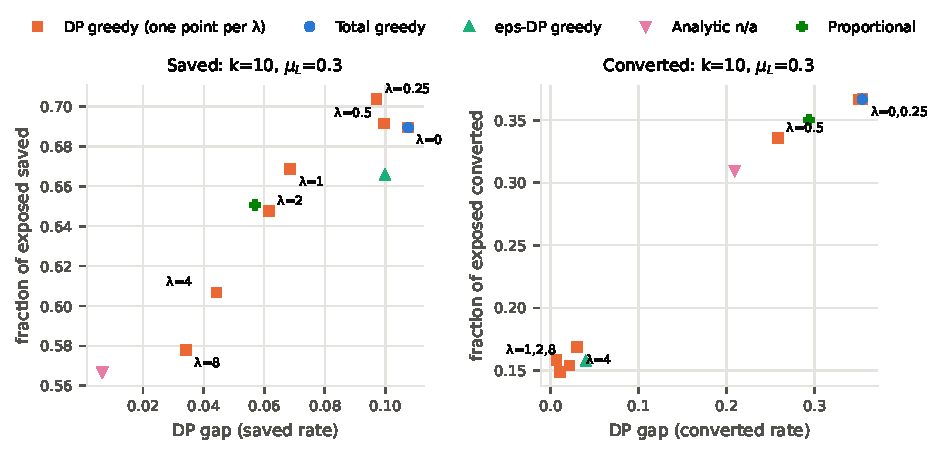
\includegraphics[width=\columnwidth]{figures/parity_pareto.pdf}
\caption{Parity experiment C: total blocked against DP gap for DP greedy with $\lambda\in\{0,0.25,0.5,1,2,4,8\}$ (one point per $\lambda$; labels merge near-identical points), at $k=10$, $\mu_L=0.3$, with the other methods for reference. Setup in Section~\ref{sec:setup}.}
\label{fig:parity-pareto}
\end{figure}
